\chapter{Introduction}\label{chap:intro}
\pagenumbering{arabic}
\setcounter{page}{1}
This document defines the specification of {\XACC} which is an extension of {\XMP} version 1.3\cite{xmp} and {\OACC} version 2.5\cite{openacc}.
{\XACC} provides a parallel programming model for accelerated clusters
which are distributed memory systems equipped with accelerators.
In this document,
terminologies of {\XMP} and {\OACC} are indicated by {\tt typewriter font}.
For details, refer to each specification\cite{xmp,openacc}.

\section{Hardware Model}
The target of {\XACC} is an accelerated cluster,
a hardware model of which is shown in Fig. \ref{fig:hardware}.

\begin{myfigure}
  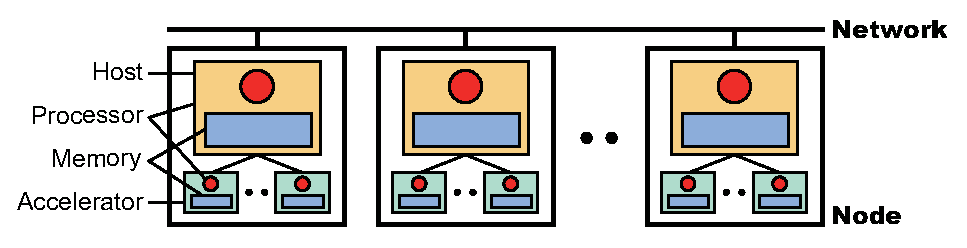
\includegraphics[scale=0.9,clip]{figs/hardware.eps}
  \caption{Hardware Model}\label{fig:hardware}
\end{myfigure}

An execution unit is called {\tt node} as with {\XMP}.
Each {\tt node} consists of a single host and multiple accelerators (such as GPUs and Intel MICs).
Each host has a processor, which may have several cores, and own local memory.
Each accelerator also has them.
Each {\tt node} is connected with each other via network.
Each {\tt node} can access its local memories directly and remote memories,
that is, the memories of another {\tt node} indirectly.
In a host,
the accelerator memory may be physically and/or virtually separate from the host memory as with the memory model of {\OACC}.
Thus,
a host may not be able to read or write the accelerator memory directly.

\section{Programming Model}
{\XACC} is a directive-based language extension based on Fortran 90 and ISO C90 (ANSI C90).
To develop applications on accelerated clusters with ease,
{\XACC} extends {\XMP} and {\OACC} independently as follow:
(1) {\XMP} extension is to facilitate cooperation between existing {\XMP} and {\OACC} directives.
(2) {\OACC} extension is to deal with multiple accelerators.

\subsection{{\XMP} Extension}
In a program using the {\XMP} extension,
{\XMP}, {\OACC}, and {\XACC} directives are used.
Fig. \ref{fig:concept} shows a concept of the {\XMP} extension.

\begin{myfigure}
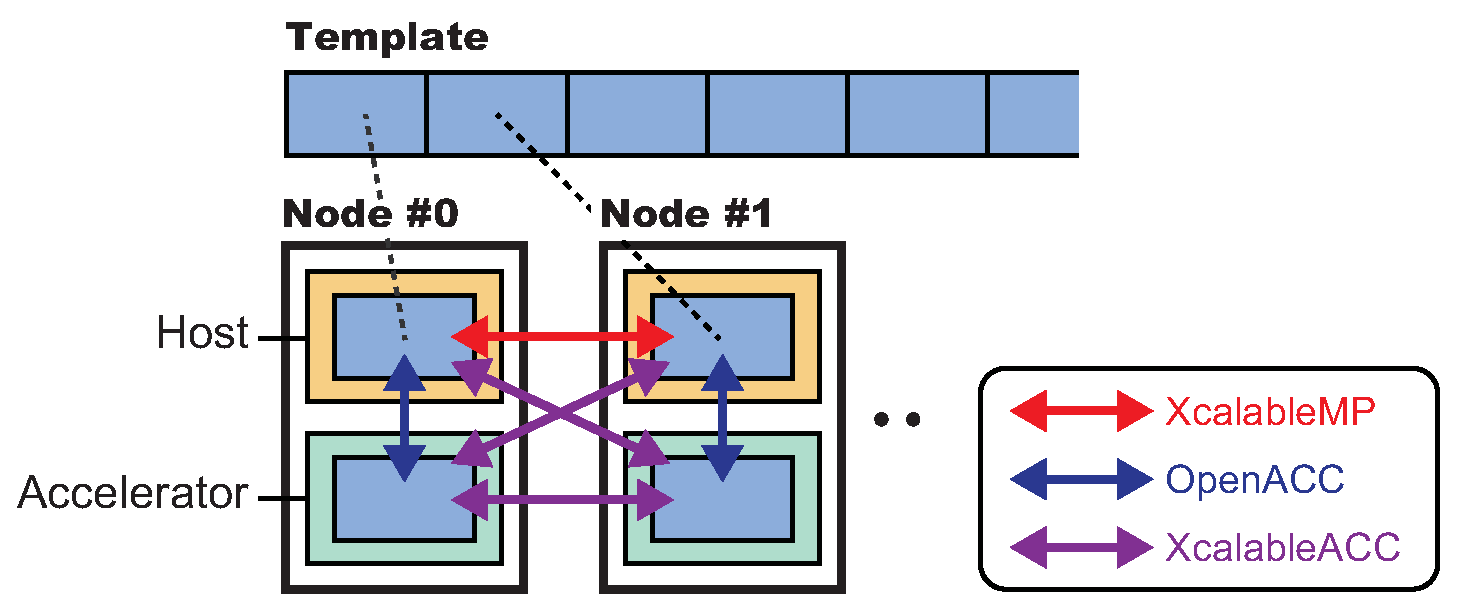
\includegraphics[scale=0.5,clip]{figs/concept.eps}
  \caption{Concept of {\XMP} Extension}\label{fig:concept}
\end{myfigure}

{\XMP} directives define a {\tt template} and a {\tt node set}.
The {\tt template} represents a global index space, which is distributed onto the {\tt node set}.
Moreover, {\XMP} directives declare {\tt distributed arrays},
parallelize loop statements and transfer data among host memories according to the distributed {\tt template}.
{\OACC} directives transfer the {\tt distributed arrays} between host memory and accelerator memory on the same {\tt node}
and execute the loop statements parallelized by {\XMP} on accelerators in parallel.
{\XACC} directives, which are {\XMP} communication directives with an {\bf acc} clause, 
transfer data among accelerator memories and between accelerator memory and host memory on different {\tt nodes}.
Moreover, 
{\tt coarray} features also transfer data on different nodes.

%The {\XMP} extension is defined to develop parallel applications with keeping the sequential code image.
Note that 
the {\XMP} extension is not a simple combination of {\XMP} and {\OACC}.
For example, 
if you represent communication of {\tt distributed array} among accelerators shown in Fig. \ref{fig:concept} by the combination of {\XMP} and {\OACC},
you need to specify explicitly communication between host and accelerator by {\OACC} and that between hosts by {\XMP}.
Moreover,
you need to calculate manually global indices of the {\tt distributed array} owned by each {\tt node}.
By contrast,
{\XACC} directives can represent such communication among accelerators directly.

\subsection{{\OACC} Extension}
The {\OACC} extension can represent offloading works and data to multiple-accelerators on a {\tt node}.
Fig. \ref{fig:concept_acc_ex} shows a concept of the {\OACC} extension.

\begin{myfigure}
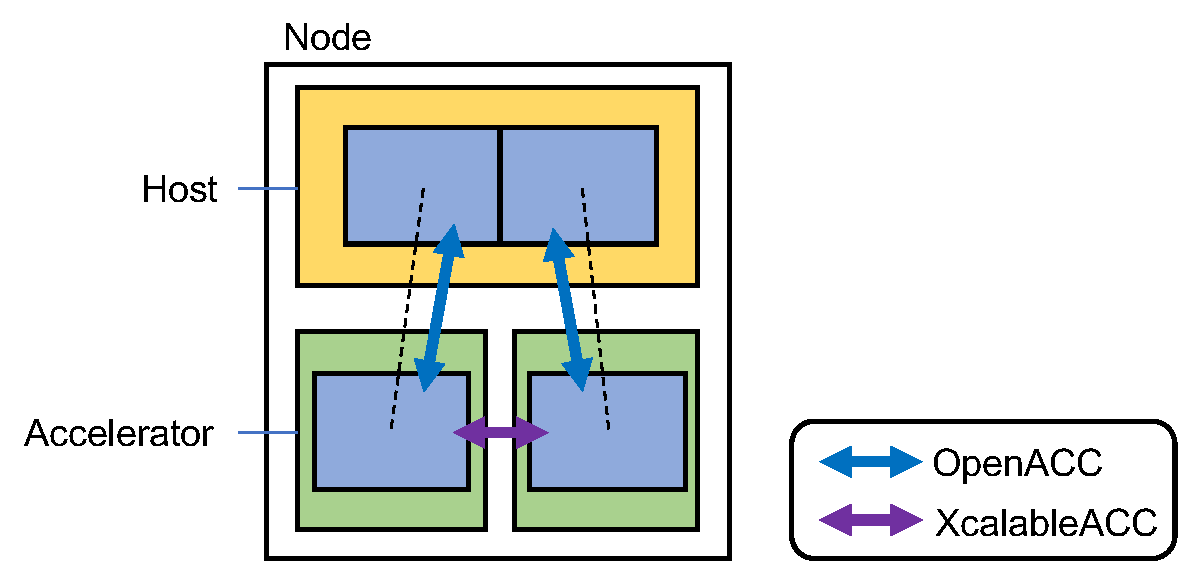
\includegraphics[scale=0.5,clip]{figs/concept_acc_ext.pdf}
  \caption{Concept of {\OACC} Extension}\label{fig:concept_acc_ex}
\end{myfigure}

{\OACC} extened directive defines a {\tt device set}.
The {\tt device set} represents a set of devices on a {\tt node}.
Futher, {\OACC} extended directives declare {\tt distributed arrays} on the {\tt device set} while maintaining the arrays on the host memory, and the directives distribute offloading loop statement and memory copy between host and device memories for the {\tt distributed-arrays}.
Moreover, {\OACC} extended directives synchronizes devices among the {\tt device set}.
{\XACC} directives also transfer data between device memories on the {\tt node}.

\section{Execution Model}
The execution model of {\XACC} is a combination of those of {\XMP} and {\OACC}.
While the execution model of a host CPU programming is based on that of {\XMP},
that of an accelerator programming is based on that of {\OACC}.
%For details, refer to each specification\cite{xmp,openacc}.

An {\XACC} program execution is based on the SPMD model, 
where each {\tt node} starts execution from the same main routine and keeps executing the same code independently (i.e. asynchronously), 
which is referred to as the replicated execution
until it encounters an {\XMP} construct or an {\XMP} extension construct.
In particular,
the {\XMP} extension construct may allocate, deallocate, or transfer data on accelerators.
An {\OACC} construct or an {\OACC} extension construct may define {\tt parallel regions}, such as work-sharing loops, 
and offloads it to accelerators under control of the host.

\section{Organization of This Document}
The remainder of this document is structured as follows:

\begin{itemize}
 \item Chapter 2: {\XMP} Extension
 \item Chapter 3: {\OACC} Extension
\end{itemize}
